\section{Related work on AUV navigation}\label{sec:lit-review}
Following paragraphs summarize the documented ways to process the sensor information in order to be able to estimate the position within the environment. 

In existing survey on underwater vehicle navigation, Kingsey \cite{kinsey06} gives a summary presenting the methods used for navigation. As introduced in \cite{kinsey06}, current vehicle position is referred as navigation state - a vector whose elements express where the vehicle is and how it is oriented in space with respect to some reference. Localization simply means finding a way to estimate navigation state vector. Naturally, sensors are providing the data for the estimation.

The simplest approach would be dead reckoning - to take the raw sensor measurements and use them directly or within a simple mathematical model that describes the vehicle dynamics. Instead, many techniques presented in literature utilize sensor data as supplementary information together with the information from the kinematic model.

Underwater navigation is using several instrumentation methods to carry out the robot localization in the sea \cite{whitcomb99}. These include transponder networks placed on the bottom of the sea, tracking systems between the ship and the underwater vehicle, and sensory devices that measure range and dynamics mounted on the vehicle itself. Each of the methods has its advantages and disadvantages. Transponder network gives accurate position information, however using it requires installing and calibrating additional equipment \cite{eustice05}.

\subsection{Kalman filtering localisation}
Some past works have already dealt with the issue of managing robot localization using Kalman filtering. Master thesis of Negneborn \cite{negenborn03} gives a useful overview of the theoretical knowledge in field of probability and estimation. Thesis also surveys the utilization of Kalman filtering for localizing vehicles in general. Emphasis is on application in robotics. Several experiments have been reported in the thesis with a detailed discussion. This work is a good starting point in learning and understanding the problem of localization on physical robots in general and, in particular, usage of Kalman filtering for that purpose.

Blain et al. \cite{blain03} study the application of Kalman filter in navigation of an underwater vehicle used for water dam inspection focusing on merging position orientation and velocity information. This algorithm uses acoustic positioning sensor together with the integration the DVL sensor (Chapter \S~\ref{chap:sensors}) measured velocities \cite{blain03} to estimate the position. Apart from reporting performance of \textit{sensor-fusion} in real application, several issues have been pointed out and dealt with in their work, such as managing asynchronous information that arrives from sensors. It is reported that Kalman filter output could be corrupted in situations when observations (sensor measurements) are subject to interruption or periodic stopping. Due to the fact that not all the sensors can be always available, it is usually necessary to be capable of adding or removing sensor observations from the system without changing the navigation algorithm. 

Asynchronous data delivery in this particular case means that the DVL sensor (Chapter \S~\ref{chap:sensors}) provides data with higher rate \cite{blain03}. Such obstacle was solved by switching to estimation procedure so that it is suitable for that particular sensor measurement scenario. This simply means that if the acoustic sensor and DVL sensor asynchronously provide new measurements, Kalman filtering is used to carry out the fusion by doing filter switching process. Each sensor has a filter process attached to it and the sensor itself defines which filter becomes active for the actual measurements. Otherwise, pure DVL velocity measurement is just integrated to update the position, as dynamic model would suggest.  
% (take into account both measurements at the correction stage).
Blain also analyses delays in absolute position measurement and validity of absolute position data if they are delayed. This effect evident in case of acoustic waves, where the real time of the measurement is current measurement time minus the time it took for the acoustic signal to arrive. It is especially visible in cases when acoustic signal moves across a longer distance. This causes a delay in data arrival. To overcome this, position estimate between two acoustic measurements is memorized. Position is meanwhile normally updated by integrating the DVL data that happen more frequently. To compensate for the time it took for the acoustic signal to arrive, timestamp of the moment when the data was produced was estimated and memorized together with the current position at the timestamp. The procedure consists of two stages: at first, a new position estimate is made using the recieved acoustic position data to update the position at the timestamp. Finally, the correction is applied on the updated position by integrating velocities that happened in meanwhile - from the timestamp till the actual time. This serves as the correction of the position estimate error influenced by significant time of flight of the signal. 

Drolet et al. \cite{drolet00} introduce a flexible localization strategy based on sensor fusion and usage of several Kalman filters arranged together in a bank. Each filter is reduced to express a simple kinetic equation. In addition, each filter processes one state - works in one ``dimension''. Idea is to integrate together sensor measurements that arrive at different time moments from different sensors. Method takes asynchronous information from sensors, manages a filter switching process so that the most recent data is used to update those filters that can be updated with such measurement \cite{drolet00}. Such sensor fusion strategy is adaptable in terms of number of sensors so that the best is taken out from the available input data, more robust to data loss. Moreover, asynchronous inputs are allowed. 

Di Massa et al. report usage of Kalman filter framework for slightly different concept of navigation that takes surrounding terrain as reference for estimating the position of the sonar (``terrain-relative navigation''), \cite{diMassa97}. In their work, sonar image is matched to the map using mean absolute difference (MAD) as the matching criterion. Matching map location is considered as the measurement of the vehicle position \cite{diMassa97}. Matching process is not entirely transparent - there are always several candidates eligible to be candidate for best matching. Thus several matchings are selected and weighted depending on how much they relate to the terrain images. Weights correspond to uncertainties in estimation theory. Quality of similarity is used to weight each measurement. Solution consists of having resulting best estimate of location \cite{diMassa97}. Information from selected matches is combined to make the best estimate. The role of Kalman filter framework is to carry out the estimation. Each of the chosen matches is considered as one measurement together with its weight as uncertainty. The filtered state is the position of the image within the map. 

Gade and Jalving introduce post processing aided navigation system deployed on a commercial underwater vehicle \cite{gade99}. Idea is that the underwater vehicle records sensor data while accomplishing mission under the sea surface (capturing images of the seabed). At the same time, a vessel is positioned on the surface receiving information of its position through the reliable Differential Global Positioning System (DGPS). After the mission is over, data are combined together with position data that was simultaneously recorded on the survey vessel located on the surface. Kalman filtering is used when merging the data. \textit{Error-state} Kalman filter \cite{gade99} is used to combine sensor measurements and their error models. Observations in case of such filter consist of the difference between measured and computed values. Instead of working directly with states, presented algorithm filters the errors, so that the ultimate position and heading estimate can be derived by subtracting the estimated errors from, as authors suggest, corresponding calculated state elements. This way, final aim of obtaining more accurate vehicle position and heading together with the tunable accuracy of such estimate \cite{gade99} contibutes in improving the accuracy of obtained seabed maps. 

Dissertation \cite{roman05} suggests how to improve the vehicle position estimation when reconstructing maps of the sea floor. Visual information of the terrain is used as the feedback that makes terrain mapping data and the vehicle navigation data more consistent. Inspiration for investigating lies in fact that map-making depends on localization quality. Navigation errors are potentially large scale particularly seriously affecting the results when mapping is vehicle-based \cite{roman05}. Existing local navigation is used together with terrain-relative measurements. Namely, terrain sub-maps are created over short periods while the vehicle works out the inaccurate localization using dead reckoning. Sub-maps are registered resulting in position measurements between two vehicle states, placing an additional constraint on the vehicle position estimates. Delayed EKF is used to merge together the measurements (``sub-map'' registrations and previously reached vehicle locations) into the navigation framework. Delayed state version of the recursive EKF enables retaining knowledge of prior platform positions.  

Yun et al. introduce simulation and present testing results of the navigation system that combines the usage of Inertial Measurement Unit (IMU) together with GPS fixes that occur less frequent and asynchronously \cite{yun00}. Asynchronous Kalman filter with six states for orientation and eight states for position estimation is implemented \cite{yun00}. Process model takes the velocities and GPS bias, models them as white noises passed through the first order systems with the time constant. Measurement consists of synchronous (periodical) velocity measurements and asynchronous DGPS information. The design of the filter for the position estimation algorithm conforms to the standard routine, with the difference that the measurement vector has different length depending on the number of available valid sensor inputs, hence it has a flexible size, but each observation updates the state vector of the fixed size \cite{yun00}. The idea of the asynchronism enables that DGPS signals are used, if available and as soon as they are available, together with the speed measurements. This way, the localization algorithm uses the most of the data that are currently available.

The usage of the stochastic estimators implies using a known model that describes system state transition from one moment to another (\textit{plant model}) and model that describes transition from state to the measurement (\textit{observation model}). Such model does not have to be the same each time. Jakuba and Yoerger \cite{jakuba03} study the way to optimize navigation by estimating the vehicle model parameters, for instance various dynamics or buoyancy coefficients that normally influence the model, but are treated as constant. Their study involves post-processing of the navigation data and heuristic estimate of these coefficients' optimal value. Real missions that applied the technique resulted in reduced noise in localization data, therefore giving clearer tracking. 

Julier and Uhlmann introduce the method that carries out nonlinear filtering \cite{julier96}. It is an alternative generalization of the KF that changes the approach of representing mean and variance of the random variable after it passes through an nonlinear transform. Their research is a quite useful and comprehensive theoretical overview of filtering in general and the role of Extended Kalman Filter (EKF) in switching to nonlinearity world. Introduced filter, later known as Unscented Kalman Filter (UKF) is regarded as more precise alternative to EKF that is, in addition, fairly easy for implementation. Julier and Uhlmann in their work point out the shortcomings of the EKF. In search of general method that would overcome the problem, instead of using proposed equations for projecting mean and covariance, a discrete set of points is chosen and projected using a chosen non-linear transformation (Section \S~\ref{sec:ukf}). Idea is to use the parameters to approximate the Gaussian distribution instead of approximating the nonlinear transformation. This way, propagation of the information is accomplished directly, and the aim is to find a way to parametrise the information about the mean and covariance of the distribution. Advantages of the filtering algorithm are in terms of precision and simplicity (no need for Jacobian derivation) with empirical results for highly nonlinear problems including vehicle control indicating as good as or better performance than EKF and higher robustness.

Wan and van der Merwe \cite{wan00} go further in exploring the concept of UKF introduced by \cite{julier96}. Their research briefly reminds of disadvantages manifested in EKF and improvements gained with the usage of UKF. UKF theoretical backgrounds, the idea itself and meaning of used variables were explained in comprehensive manner in one of the document sections. Usage of UKF was reported together with the results in different estimation problems such as nonlinear system identification, state estimation, parameter estimation and dual estimation problems \cite{wan00}. UKF according to the authors achieved higher accuracy compared with EKF in all the domains that were examined.

At this point, it is useful to make a short digression in order to give more details on EKF and UKF.

\subsubsection{Extended Kalman Filter} \label{sec:ekf}
System can be described with set of states that evolve in time according to mathematical functions that are nonlinear in many applications. Table ~\ref{tab:system} gives an overview, categorizing systems as linear or nonlinear. Nonlinear state prediction would use previous state estimate and mean value of the process noise:
\begin{equation}
\vect{\hat{x}}(k \mid k-1) = f(\vect{\hat{x}}(k-1), \vect{u}(k), 0)
\label{eq:state-pred-nonlin}
\end{equation} 
EKF is intended for solving sub-optimal state estimation of a nonlinear system. The main characteristic of EKF is that it analytically approximates - linearises - the process and measurement functions ($f()$ and $h()$, Table ~\ref{tab:system}). Linearisation implies approximating these functions with their first derivative around current prediction, similarly as the ordinary functions are approximated with Taylor polynomials of first degree. In this case, derivation is slightly more complex since model functions $f()$ and $h()$ take several input vectors and output the resulting vector. Hence, the derivation will consist of partial derivation of process per state input vector (Equation ~\ref{eq:der-proc-state}) and per noise input vector (Equation ~\ref{eq:der-proc-noise}). And partial derivation of measurement function per state (Equation ~\ref{eq:der-mes-state}) and measurement noise (Equation ~\ref{eq:der-mes-noise}). Partial derivatives themselves will be Jacobian matrices considering that vector is derived per vector. 
\begin{equation}
\vect{F}(k) = \frac{\partial f}{\partial x} (\vect{\hat{x}}(k \mid k-1), \vect{u}(k), 0)
\label{eq:der-proc-state}
\end{equation} 
\begin{equation}
\vect{W}(k) = \frac{\partial f}{\partial n} (\vect{\hat{x}}(k \mid k-1), \vect{u}(k), 0)
\label{eq:der-proc-noise}
\end{equation}
\begin{equation}
\vect{H}(k) = \frac{\partial h}{\partial x} (\vect{\hat{x}}(k \mid k-1), 0)
\label{eq:der-mes-state}
\end{equation} 
\begin{equation}
\vect{V}(k) = \frac{\partial h}{\partial m} (\vect{\hat{x}}(k \mid k-1), 0)
\label{eq:der-mes-noise}
\end{equation}
Subsequently, filtering process can be treated similarly as classic, discrete linear Kalman filter introduced in previous section. 
\begin{algorithm}%[h!]
\caption{The Discrete Extended Kalman Filter} \label{alg:ekf}
\begin{algorithmic}
\REQUIRE $E\lbrace \vect{x}(0) \rbrace = \vect{x}(0) = \vect{\hat{x}}(0)$
\COMMENT{initialize state}
\REQUIRE $\vect{P}(0) = \delta_{jk} \vect{P_{0}} $ 
\COMMENT {initialize covariance}
\LOOP 
	\STATE $k \Leftarrow k+1$ 
	\STATE $\vect{\hat{x}}(k \mid k-1) = f(\vect{\hat{x}}(k-1), \vect{u}(k), 0)$
	\COMMENT {state prediction}
	\STATE $\vect{P}(k \mid k-1) = \vect{F}(k) \vect{P}(k-1) \vect{F}^{T}(k) + \vect{W}(k) \vect{Q} \vect{W}^{T}(k)$
	\COMMENT {state prediction uncertainty}	
	
	\STATE $\nu = \vect{z}(k) - h(\vect{\hat{x}}(k \mid k-1), 0)$	
	\COMMENT {innovation}
	\STATE $\vect{S} = \vect{H}(k) \vect{P}(k \mid k-1) \vect{H}^{T}(k) + \vect{V}(k) \vect{R} \vect{V}^{T}(k)$	
	\COMMENT {innovation uncertainty}	
	\STATE $\vect{K} = \vect{P}(k \mid k-1) \vect{H}^{T}(k) \vect{S}^{-1}$	
	\COMMENT {``Kalman gain''}	
	
	\STATE $\vect{\hat{x}}(k) = \vect{\hat{x}}(k \mid k-1) + \vect{K} \nu$
	\COMMENT {state correction} 
	\STATE $\vect{P}(k) = (\vect{I}-\vect{K}\vect{H}(k))\vect{P}(k \mid k-1)$
	\COMMENT {state correction uncertainty}
	\RETURN $\vect{\hat{x}}(k), \vect{P}(k)$
\ENDLOOP
\end{algorithmic}
\end{algorithm}
Process model mathematically describes how the state changes for the given input (Equation ~\ref{eq:state-pred-nonlin}). Essential invention in EKF algorithm is the linearisation of the given function around current state mean and variance which further results in estimation process similar to the one described for linear Kalman filter.
%There can be various number of states and all of them are grouped together in the state vector. Navigation system could, for instance, group together position coordinates and orientation angles in the state vector. If the system is considered as discrete, transition from one discrete value of the state vector to the next one, is described with the function $f$ called process model, equation ~\ref{eq:state-transition}, where the current state, $x(k+1)$, is calculated using the process model with previous state ($x(k)$), current input ($u(k+1)$) and process noise ($v(k+1)$) as arguments. In other words, 
%Thus, our system is not entirely an unknown black box once a linear Kalman Filter(KF) is attached to it. A hint about its dynamics is known in form of process model. The only information available once the filtering starts, are its control inputs ($u$) and a set of observations ($z$). equation associates observations with the state. Similarly as shown in ~\ref{eq:state-transition}, $x$ and $u$ present the state, while $w$ represents the additive measurment noise and function $h$ observation model \cite{julier96}.
%\begin{equation}
%\begin{split}
%E \left[ \vect{v}(i) \vect{v}^{T}(j) \right]  = \delta_{ij} \vect{Q}(i) \\
%E \left[ \vect{w}(i) \vect{w}^{T}(j) \right]  = \delta_{ij} \vect{R}(i) \\
%E \left[ \vect{v}(i) \vect{w}^{T}(j) \right]  = \vect{0}, \forall i,j
%\end{split} 
%\label{eq:noise}
%\end{equation}
%% this could go to methodology
% This would mean that the mean and the variance of the state are measurable. Prediction in case of moving vehicle is calculated based on previous vehicle location and dead reckoning. One of its particularly useful features is the ability to combine together sensor measurements in mathematical form such that the solution is best possible estimate of the mean and the variance. relationship between previous estimation $()$ and the current

Kalman gain determines the importance of each new observation $\vect{z}(k)$. Essentially - it expresses how much we allow the measurement to influence the change of the predicted state at the correction stage. According to the state correction formula (Algorithm ~\ref{alg:ekf}), it is determined by the values of matrices $Q$ and $R$ which represent process noise covariance and the measurement noise covariance (uncertainty), respectively. Values contained in $\vect{K}$ takes the range between $0$ and $1$ with zero $(0)$ meaning that we use only prediction as the estimation and give no importance to the measurement. One $(1)$ on the other hand, means that we give all the importance to the measurement.% consider direct measurement as the only important one.   fairly realistic

Real world models are rarely linear. The motive for developing the Extended Kalman Filter is based on the adaptation of the linear Kalman Filter for dealing with nonlinear problems. However, it is possible that EKF significantly declines the performance quality \cite{julier96}. When making a prediction of state, observation or uncertainty of any of those for nonlinear systems, linearisation can introduce errors. The inaccuracies of the EKF estimates are caused by truncating errors in Taylor series when making an approximation. One example of such case is given in \cite{julier96} where the simulated object trajectory follows circular path. The reason for failing in prediction stage in such scenario is in linear approximations that EKF, naturally, uses when predicting the next state and its characteristics.
%%%%%%%%%%%%%%%%%%%%%%%%%%%%%%%%%%%%%%%%%%%%%%%%%%%%%%
\subsubsection{Unscented Kalman Filter (UKF)}\label{sec:ukf}
%When the system and observation model are nonlinear functions, EKF performs bad. One particular case of low performance is presented in \cite{julier96} where the filtering of covariance turns out to be imprecise. % (or possibly randomly) 
UKF refers to usage of the unscented transform in EKF framework \cite{julier00, wan00, ristic04}. Instead of propagating random Gaussian variable through nonlinear transform functions $f()$ and $g()$, UKF deterministically chooses set of sample points, large enough to capture the distribution of the variable. Idea is that the probability distribution is approximated using weighting of the propagated samples rather than the approximation of the nonlinear function. Distribution is modelled as Gaussian, thus represented with mean and variance, as it is general principle with Kalman filtering. The role of Unscented Transform (UT) is in providing the technique for estimating statistical parameters of the Gaussian random variable (GRV) that undergoes nonlinear transform (Figure ~\ref{fig:gauss-transform}). UT provides the pattern for sample selection and scheme for estimation of statistical parameters (such as mean and variance for GRV) after nonlinear transformation of selected samples.

\T{Unscented transformation (UT). } Provides a method for calculating statistics of a random variable that undergoes nonlinear transform. Gaussian random variable $\vect{a}$ of vector length $L$, mean value $\vect{\bar{a}}$ and variance $\vect{P}_{a}$ is passed on to a nonlinear function $g()$ that eventually creates another random variable, $\vect{b}$ of the same length.
$$ \vect{b} = g(\vect{a}) $$   
The aim is to estimate mean and variance of the variable after the transformation. Such solution will be useful since the nonlinearities in process model can be significant. First order Taylor approximation was used within EKF for such task.

UT defines the set of $2L+1$ samples $(A_{i})$ which are capturing the distribution (Figure ~\ref{fig:sigma-samples}). Each sample has a weight coefficient $(W_{i})$ attached to it. Weights are normalized so that they all sum up to one. Weights will be used in calculation of the mean and variance of obtained variable $\vect{b}$: $\vect{\bar{b}}$ and $\vect{P}_{b}$. Samples and their respective weights are formed using equations:
\begin{eqnarray}
\begin{array}{l c r}
\vect{A}_{i} = \vect{\bar{a}}, & \vect{W}_{i} = \frac{k}{L+k}, & i = 0 \\
\vect{A}_{i} = \vect{\bar{a}}+(\sqrt{(L+k)\vect{P}_{a}})_{i}, & \vect{W}_{i} = \frac{1}{2(L+k)}, & i = 1,...,L \\
\vect{A}_{i} = \vect{\bar{a}}-(\sqrt{(L+k)\vect{P}_{a}})_{i-L}, & \vect{W}_{i} = \frac{1}{2(L+k)}, & i = L+1,...,2L \\
\end{array}
\label{eq:ut-sampling}
\end{eqnarray}
with parameter $k$ setting the distance of sample points from $\vect{a}$ (Figure ~\ref{fig:sigma-samples}). $(\sqrt{(L+k)\vect{P}_{a}})_{i}$ presents $i$-th row of matrix square root of $(\sqrt{(L+k)\vect{P}_{a}})_{i}$. Eventually, each selected sample is substituted in nonlinear function $g()$, resulting in samples $\vect{B}_{i} = g(\vect{A}_{i})$ , $i = 0 ,..., 2L$. Mean value (first moment) and covariance (second moment) of the obtained random variable are:
\begin{equation}
\begin{array}{l r}
\vect{\bar{b}} = \sum_{i=0}^{2L} \vect{W}_{i} \vect{B}_{i},   &
\vect{P}_{b} = \sum_{i=0}^{2L} \vect{W}_{i} (\vect{B}_{i} - \vect{\bar{b}}) (\vect{B}_{i} - \vect{\bar{b}})^{T}
\end{array}
\label{eq:ut-estimate}
\end{equation}
\begin{equation}
\vect{b} = g(\vect{a}) = \left[ \begin{array}{c} \vect{a}(1) \cos \vect{a}(2) \\ \vect{a}(1) \sin \vect{a}(2) \end{array} \right]
\label{eq:2cart}
\end{equation}
The concept was explained through an example \cite{ristic04}. Two-dimensional GRV was used to express the position in polar coordinates. Such position information contains number of samples of range (distance) and bearing (angle). An example of nonlinear transformation where polar coordinates are transferred into Cartesian coordinates using function $g()$ (Equation ~\ref{eq:2cart}) was analysed. Original set of samples was shown in Figure ~\ref{fig:original}. Figure ~\ref{fig:lin-approx} shows estimation of the mean and covariance using first order linearisation (Jacobian) of $g()$ - scheme that is included in standard EKF. It is visible that both mean and covariance estimates have errors. Although dissonant, EKF still performs well in practise implying the nonlinearities are moderate \cite{ristic04}. In search of more accurate estimate, or at least less prone to nonlinearity, UT was investigated. Figures ~\ref{fig:sigma-samples} and ~\ref{fig:unsc-transform} demonstrate the usage of UT. At first, samples have been computed (Equation ~\ref{eq:ut-sampling}), transferred into Cartesian using function $g()$ and their statistic moments revealed using weighted average functions (Equation ~\ref{eq:ut-estimate}). Compared with linear approximation, UT proves to be more accurate. It emulates nonlinarities of the prediction model better.

UKF, similarly as other Kalman filtering algorithms consists of two independent stages of prediction and update. Both stages utilize UT and its features. GRV, similar with the one from the example is used to store together state, process noise and measurement noise variables - making altogether an \textit{augmented state} vector ~\ref{alg:ukf}.

Augmented state provides GRVs that will be sampled, weighted and propagated through nonlinear process $(f())$ and measurement $(h())$ functions as a part of prediction and correction stage. After each correction, UKF will hold an estimate of current mean and variance, ready to continue with recursion (Algorithm ~\ref{alg:ukf}).   

\begin{figure}%[htp]
  \begin{center}
    \subfigure[Original Gaussian random variable samples of range and bearing.]
    {\label{fig:original}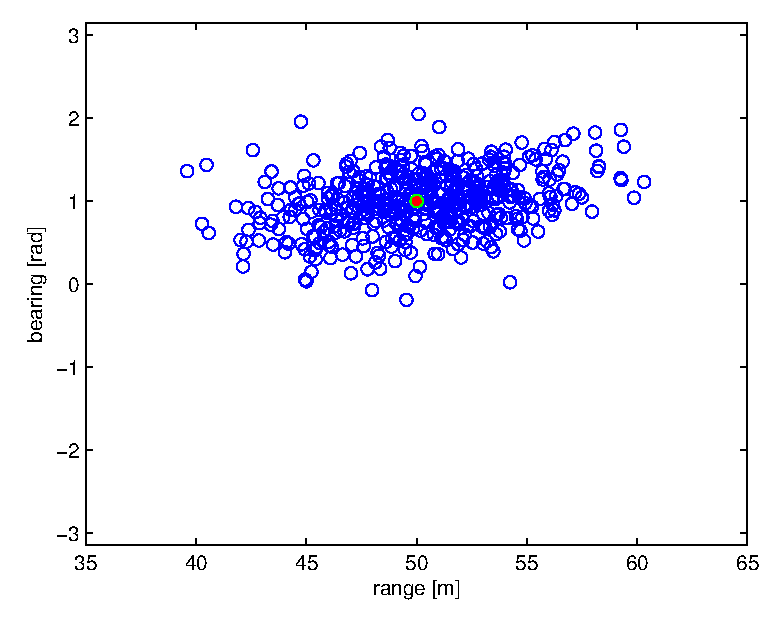
\includegraphics[width=0.40\textwidth]{kalman/fig/orig.eps}}
    \subfigure[Gaussian variable after nonlinear transform with mean and variance (ellipse) estimated using linearisation of the transform.]
    {\label{fig:lin-approx}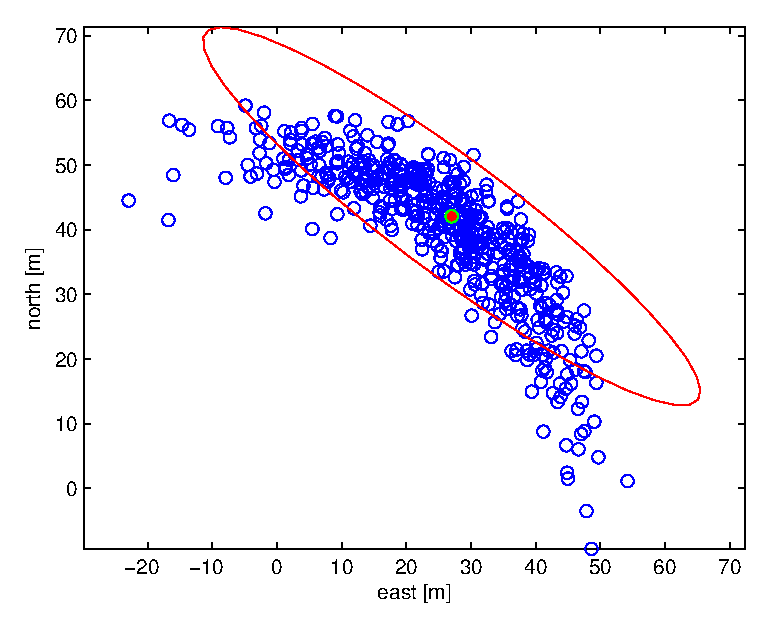
\includegraphics[width=0.40\textwidth]{kalman/fig/linear.eps}}      \\
    \subfigure[Original Gaussian random variable with samples selected by unscented transform algorithm.]
    {\label{fig:sigma-samples}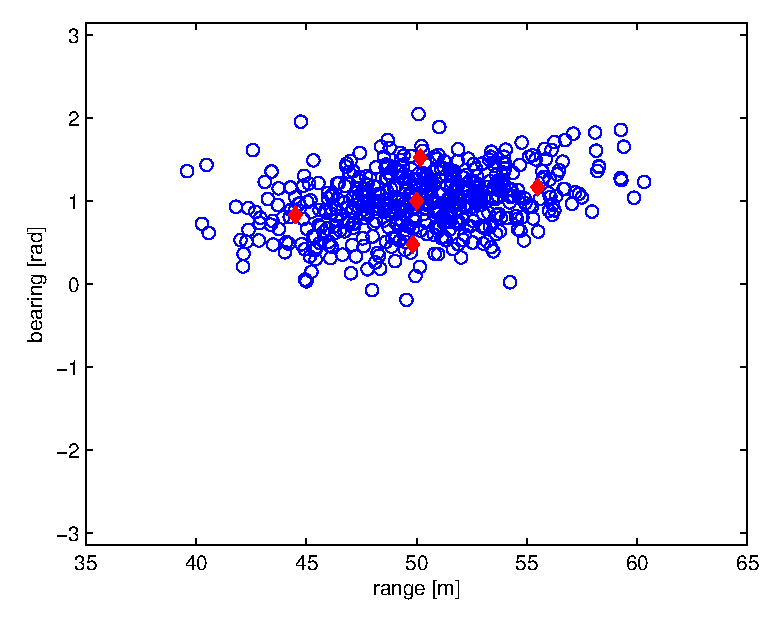
\includegraphics[width=0.40\textwidth]{kalman/fig/orig-samples.eps}}
    \subfigure[Gaussian variable after nonlinear transform with mean and variance (ellipse) estimated using unscented transform.]
    {\label{fig:unsc-transform}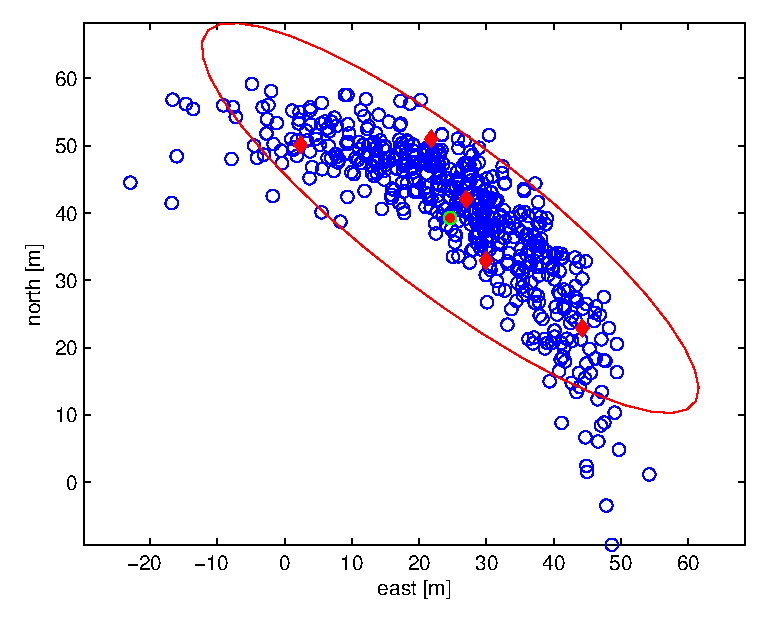
\includegraphics[width=0.40\textwidth]{kalman/fig/unscented.eps}}
  \end{center}
  \caption{Nonlinear transformation of a Gaussian random variable and estimation of its statistical parameters - mean and variance, using linearisation approximation and unscented transform.}
  \label{fig:gauss-transform}
\end{figure}

Calculation-wise, the whole procedure is fairly easier compared with linearisation algorithm since there is no need for calculating the Jacobian or Hessian, total number of computations stays the same and it is easier to improvise with the algorithm with constrains or parameters which define the way samples are selected. In addition, UT shown in example (Figure ~\ref{fig:gauss-transform} ) handles the whole distribution and its transformation by tracking only five samples. Higher dimensionality of GRV would result in more samples taken. However that number is still reasonably small compared with Monte Carlo methods. The only difficulty in implementation could be the non-trivial solution of the square root of the matrix as the necessary stage in unscented transform computation (Equation ~\ref{eq:ut-sampling} ).
\begin{algorithm}%[h!]
\caption{The Discrete Unscented Kalman Filter} \label{alg:ukf}
\begin{algorithmic}
\REQUIRE $\vect{\hat{x}}(0) = E\lbrace \vect{x}(0) \rbrace$
\COMMENT{initialize state}
\REQUIRE $\vect{P}(0) = \delta_{jk} \vect{P}_{0} $ 
\COMMENT {initialize covariance}
\REQUIRE $\vect{\hat{x}}^{aug}(0) = \left[ \begin{array}{c} \vect{\hat{x}}^{x}(0) \\ \vect{x}^{n}(0) \\ \vect{x}^{m}(0) \end{array} \right]
                                  = \left[ \begin{array}{c} \vect{\hat{x}}(0) \\ \vect{0} \\ \vect{0} \end{array} \right] $ 
\COMMENT{init. augmented state: state + process noise + meas. noise}
\STATE   $L = length(\vect{\hat{x}}^{aug}) \; k = const$
\COMMENT{augmented state length and $k$ parameter set}
\REQUIRE $\vect{P}^{aug}(0) = \left[ \begin{array}{ccc} \vect{P}_{0} & \vect{0}     & \vect{0} \\ 
															\vect{0} & \vect{P}_{n} & \vect{0} \\
															\vect{0} & \vect{0}     & \vect{P}_{m} \end{array} \right] $ 
\COMMENT{initialize augmented state covariance}
\LOOP
	\STATE $k \Leftarrow k+1$
	\STATE $\vect{A}^{aug}(k-1) = \left[\vect{\hat{x}}^{aug}(k-1) \vect{\hat{x}}^{aug}(k-1)\pm \sqrt{(L)\vect{P}^{aug}(k-1)}  \right] $
	\COMMENT {compute samples - unscented transform}
	\STATE   $ \vect{W}_{i}, \; i = 0,...,2L $
	\COMMENT {compute weights}
	\STATE   $\vect{A}^{x}(k \mid k-1) = f(vect{A}^{x}(k-1), vect{A}^{n}(k-1)) $
	\COMMENT {nonlinear process model}
	\STATE	 $ \vect{\hat{x}}(k \mid k-1) = \sum_{i=0}^{2L} \vect{W}_{i} \vect{A}^{x}_{i}(k \mid k-1) $
	\COMMENT {state prediction}
	\STATE   $ \vect{P}(k \mid k-1) = \sum_{i=0}^{2L} \vect{W}_{i} (\vect{A}^{x}_{i}(k \mid k-1) - \vect{\hat{x}}(k \mid k-1)) 
																   (\vect{A}^{x}_{i}(k \mid k-1) - \vect{\hat{x}}(k \mid k-1))^{T} $
	\COMMENT {state prediction uncertainty}
	\STATE   $\vect{Z}(k \mid k-1) = h(vect{A}^{x}(k-1), vect{A}^{m}(k-1)) $
	\COMMENT {nonlinear measurement model}
	\STATE   $\vect{\hat{Z}}(k) =  \sum_{i=0}^{2L} \vect{W}_{i} \vect{Z}_{i}(k \mid k-1)$
	\COMMENT {measurement prediction - unscented transform}
	\STATE   $\vect{P}_{zz} =  \sum_{i=0}^{2L} \vect{W}_{i} (\vect{Z}_{i}(k \mid k-1)-\vect{\hat{Z}}(k)) 
															(\vect{Z}_{i}(k \mid k-1)-\vect{\hat{Z}}(k))^{T}$
	\STATE   $\vect{P}_{xz} =  \sum_{i=0}^{2L} \vect{W}_{i} (\vect{A}_{i}(k \mid k-1)-\vect{\hat{x}}(k \mid k-1))
															(\vect{Z}_{i}(k \mid k-1)-\vect{\hat{Z}}(k))^{T}$
	\STATE   $\vect{K}      = \vect{P}_{xz} \vect{P}_{zz}^{-1}$
	\STATE	 $ \vect{\hat{x}}(k) = \vect{\hat{x}}(k \mid k-1) + \vect{K} (\vect{z}(k) - \vect{\hat{Z}}(k))  $
	\COMMENT {state correction}
	\STATE   $ \vect{P}(k) = \vect{P}(k \mid k-1) - \vect{K} \vect{P}_{zz} \vect{K}^{T} $
	\COMMENT {state correction uncertainty}	
	\RETURN $\vect{\hat{x}}(k), \vect{P}(k)$
\ENDLOOP
\end{algorithmic}
\end{algorithm}

\subsection{Monte Carlo-based filtering methods}
Monte Carlo methods, based on repeated random sampling as a part of the results computation are covered in several works, mostly dealing with Particle Filters (PF). Gordon et al. enclose \textit{bootstrap filter} \cite{gordon93}, also known as Particle Filter (PF) - a recursive algorithm based on representing state vector as set of random samples which are updated and propagated. Update stage of such algorithm uses Bayes rule, however the sampling strategy implies that the state space grid is not necessary the samples are localized in regions of high probability density \cite{gordon93}. Arulampalam et al. review Bayesian algorithms for nonlinear or non Gaussian problems. The emphasis of the review is on Particle Filters (PF), their features, variants and, finally, inevitable comparison with the standard EKF \cite{arulampalam02}. Doucet in his book on Monte Carlo methods \cite{doucet01} focuses on creating an broad summary of theory and various applications of bootstrap filters, optimal Monte Carlo filters and Particle Filters. Common feature of both ``Unscented'' and ``Monte Carlo Method'' estimation techniques is the sampling phenomenon. By using sampling, linearisation of plant and observation models is avoided, hence the cause of approximation error that existed in EKF-based methods is cancelled this way. PF can handle non Gaussian and and nonlinear processes, particularly exhibited in AUV models. Moreover, PF does not need to have the initial information about the state. Sampling techniques, particularly PF, have been recently and increasingly applied as tool for navigation of an underwater vehicle.

Karlsson et al. study a sea navigation method that relies on the underwater maps (depth map) and sonar measurements that support the navigation system \cite{karlsson02}. Particle Filter is used for state estimation. Since the problem of underwater navigation using depth map is nonlinear, sequential Monte Carlo methods are used, therefore state probability density is approximated with set of particles where each particle has a location and weight assigned to it. Both values reflect the value of the density of the region in the state space \cite{karlsson02}. Hence, instead of updating mean and covariance of the state, particle location and the weight of each particle are updated with each observation using sampling importance resampling (SIR) algorithm \cite{karlsson02}, \cite{gordon93}. Prior to navigation, terrain map (reference) was created using sonar depth measurements together with the Differential GPS measurements and the obtained grid was used for navigation. Moreover, the usage of Cram\'{e}r-Rao bound was investigated in tasks such as INS system design, sensor performance or even the amount of control of that is needed for the navigation. This work presents a successful application of particle filtering for underwater navigation.

Above-mentioned work of Di Massa \cite{diMassa97} presents navigation guided by the depth measured with bathymetric sonar. Map-matching with digital bathymetric map stored on-board has been accomplished using the Probabilistic Data Association Filter (PDAF) - a recursive algorithm similar to Kalman filter, designed for one target of interest and several measurements of the target state available each time step \cite{diMassa97}. Position within the bathymetric map was stored as the state vector that was filtered. Results proved that such navigation is possible and that having a more diverse sea floor leads to more accurate navigation.

Maurelli et al. \cite{maurelli08} propose a particle filter based underwater vehicle localization method for both structured and unstructured environment. Mechanically scanned profiling sonar is used as sensory device which provides information on distances from surrounding objects in environment. There is no information about initial position and orientation of the vehicle prior to localization. The work explores the possibility of dealing with dynamical situations when carrying out the localization results in movements of the vehicle that contribute in improving the particle filter algorithm output - active localisation. Improvements of the PF algorithm concern computational efficiency and effective way of treating state space in order to recover from wrong convergence when using PFs. Simulation and real experimental results are available.

\subsection{GPS aided localisation}
Caiti explored localization technique that uses floating acoustic buoys provided with GPS connection \cite{caiti05}. Idea is that buoys supply the vehicle with their GPS location by emitting the information at regular time intervals. This way, vehicle can calculate the time of flight of the acoustic signal and locate itself with respect to the buoys. In such constellation, additional equipment has to be installed and maintained. Furthermore, acoustic signals are not reliable, their range is limited and signals not always available. 

Erol \cite{erol07} proposes a method for localization of the network of underwater sensors using single AUV as aiding device. This is just one of the examples of utilization of knowledge on AUV location. The aim is to use it to maintain localization of group of other objects in the water such as acoustic sensors. It is a system where AUV initially and occasionally receives GPS signals while being on the surface. Once the GPS location is received, vehicle dives to a certain depth and follows the defined path in between the sensor network. Set of freely deployed acoustic sensors is receiving messages containing coordinates from the vehicle, since the vehicle maintains updating its position using dead reckoning combined with occasional GPS correction. Emphasis is on algorithms for distance estimation so that proper values for sensor coordinates can be passed on to sensor network localization algorithm.
\subsection{Localisation using \textit{a-priori} map}
Eustice experiments with re-navigation for AUVs \cite{eustice05towards}. The aim is to use a-priori given, ship derived bathymetric maps to reduce dead reckoning drift by comparing ship-derived depth map with the depth map created by vehicle. The difference between them is used as correction, a tool for removing long-term drift. 

Williams is presenting a new method that uses terrain features for aiding the tracking of underwater vehicles in unstructured environments \cite{williams06}. Benefit of such research lies in creating a vehicle capable of adopting to terrain changes therefore capable of being reliably deployed for longer time deep underwater, on a real task, with real environment. This work is revolutionary in solving the position update for a vehicle. Most common solution is the usage of acoustic transponders and triangulation algorithm as already exposed in Chapter \S~\ref{chap:capabilities}. Williams uses a priori elevation maps of the sea floor, recorded by ships. Depth information obtained from such mapping is assisting the localization process. Localization uses Monte Carlo methods, particularly PF, to manage map-based localization with position and velocity kept within state vector. Non-Gaussian estimates obtained using particles are bounded using depth and altitude observations by using range information to rule out less probable particles. Update is accomplished by resampling the particle distribution with respect to likeliness that the observation detected is received, given the sample of the state space \cite{williams06}. Apart form dealing with non-Gaussian estimates, advantages of such method include ability to track more than one possible target placement, which proves to be useful feature when handling map-based information.  
%%%%%%%%% A-PRIORI LANDMARKS CONSTRUCTED USING SENSOR DATA %%%%%%%%%%%%
Newman and Durrant-Whyte propose a navigation filter which uses inertial measurement unit (IMU) and sonar to carry out the terrain-aided navigation \cite{newman98}. IMU is used to measure the kinematic parameters such as accelerations and rotations with respect to body frame, while sonar measures absolute distances and orientations with respect to the world frame. In such configuration, sonar system does the correction of the noise-corrupted, drift-prone position indicated by IMU. Standard Kalman filter is used to integrate different sensor measurements with a-priori dynamics model of the vehicle. Sonar observations are processed with target extraction algorithm isolating terrain beacons. Map is simultaneously created during the vehicle mission. It map serves as the representation of the world and contains distinctive features from environment. Map is intended to be a sparse world representation, containing least possible but still enough information (features) to make a reference to and it is derived from estimation of the floor gradient using sonar measurements. Pose observation is defined relative to features from the map that correspond to features from the real world.

Similarly, Williams et al. present the results of operational algorithm that processes sonar scans in order to extract robust features of the environment further used to build an environment map consisting of those features \cite{williams00}. The vehicle location is estimated within the built environment map. The work is an example of practical application of SLAM (Section \S~\ref{sec:slam}).

Another contribution of Eustice \cite{eustice05exactly}, based on vehicle localization with simultaneous terrain-features map creation (SLAM), reports usage of delayed state model. Robot movement is observed with respect to its previous position. Benefit of the delayed state framework lies in having precisely sparse information matrix. Main idea of the work is that, unlike previous algorithms, sparseness of the SLAM information matrix used in localization is guaranteed, not approximated.
%%%%%%%%% TERRAIN-AIDED WHEN TASK IS ACHIEVED %%%%%%%%%%%%
%%%%%%%%% OTHER THAN TIME-OF-FLY %%%%%%%%%%
%%%%%%%%% OPTICAL SENSING %%%%%%%%%%%%%
\subsection{Optical sensing}
Tena Ruiz investigates terrain aided localization of an AUV from the perspective of Simultaneous Localization and Mapping (SLAM) \cite{ruiz01}. Sonar device is used to sense the environment and its readings are used to find targets located not far from the vehicle. SLAM algorithm uses detected targets together with a vehicle model to simultaneously construct the environment map and localize the vehicle using filtering. Multiple Hypothesis Tracking Filter is adjusted to the SLAM framework. Necessary step of matching the sonar images with environment targets was accomplished by extracting the features and associating them with the sonar recordings by calculating a score that expresses the probability of a certain target causing a certain sonar output. 

Williams presents the results of sonar usage together with the vision based system in SLAM algorithm for terrain-aided navigation \cite{williams04}. Seabed covered with visually distinctive textured reefs was used in estimating vehicle motion and creating a map of the reef structure.  

Eustice proposes several works on vision based localisation for AUVs in an unstructured undersea environment. Framework presented in \cite{eustice04} blends together sensor data and camera measurements in order to determine the relative pose. The final aim is to concurrently determine the vehicle position and the past trajectory \cite{eustice04}. Augmented state Kalman filter is used to filter out the pose of the vehicle. History of poses defines vehicle trajectory. Registered images obtained with camera provide spatial constraints for the position hence providing the necessary feedback for pose estimation. Moreover, the registration of the image pairs is more robust compared with the situation when only camera is used for sensing. The other vision based SLAM approach \cite{eustice05} addresses the problem of localization within large areas. Precise localization is a prerequisite for high resolution underwater imaging of large objects placed on the sea-bed \cite{eustice05}. Precise navigation would enable decent coverage of the spacious site of interest which is mission task. Proposed solution uses a vision-based SLAM approach together with vehicle's inertial sensors' measurements. The originality of the paper is that it suggests a genuine solution for evaluating covariance bounds within the EKF used for filtering SLAM information. 

Carreras \cite{carreras03} experiments with the usage of visual information for underwater robot localisation within the pool with clear visibility. This method is not intended for ocean environment, however, it is useful from the computer-vision side and potentially a tool to aid video mosaicking algorithms. Camera is mounted on the vehicle and used to simultaneously record the bottom of the tank covered with the coded pattern. This way, structured environment is used for, map-based 3D localisation of the vehicle. Number of computer-vision related matters are examined, such as: necessary camera calibration, filtering methods, landmark detection. Localisation performance is reported to be high, with high computation rate and, importantly, prone to drift. Hence, reliable position information is good enough to derive the velocity estimates from it. In addition, work contains the analysis of the source of localisation errors and real time application examples.  
%%%%%%%%%%%%%%%% SLAM BASED %%%%%%%%%%%%%%%%%%%%%%%%%%%
\subsection{Simultaneous location and mapping}
In order to deal with SLAM issues, several methodologies are covered in literature. View-based approach generally relies on registering different types of imagery: optical imagery or depth imagery in order to establish spatial constraints that are vision-based, therefore, not prone to drift error (\cite{garcia01, eustice05towards, roman05}). This approach does not include precise representation of features. SLAM frameworks that, however, use features (feature-based) instead of view are reported in (\cite{williams04, ruiz01}).
%%%%%%% COMMUNICATION COOPERATIVE NAV PAPERS %%%%%%%%%%
\subsection{Cooperative navigation}
The dissertation of Bahr (\cite{bahr08}) focuses on cooperative navigation, and furthermore, general background on localisation is surveyed. Bahr proposes a probabilistic-based algorithm, particularly tailored to the underwater environment. Cooperation in navigation is already available in air or the surface of the Earth. The work focuses on cooperative localization where different vehicles, arranged in group, communicate between each other. To accomplish cooperative localization, algorithm estimates inter vehicle range, resulting in position and the uncertainty of the position, then exchanges that information with other vehicles. Main idea is to exchange  localisation-related information. The whole process consists of data acquisition and data processing stage. Forward propagation of position information causes more than one solution available. Further data processing gives an estimate of the location by processing all the possibilities. Stated advantages of such approach are that, apart from having more than one vehicle, no additional infrastructure is necessary \cite{bahr08}. Everything comes down to the usual sensor and communication package already available on vehicles\cite{bahr08}. 
%They use it together with the localisation data received from the other vehicles to make corrections of the position and position covariance.

Fallon et al. \cite{fallon10} describe the implementation of the cooperative localisation algorithm that works within group of AUV vehicles, aided with the position information from the autonomous surface vehicle to bound the estimation errors. Instead of the usage of expensive navigation sensors for communicating under the water surface, an approach where cooperation with one surface vehicle was suggested. Surface vehicle is intended to contribute with accurate position information. One of the contributions of the work is a trial of EKF localisation run on AUV and supported by the surface vehicle moving along with the AUV. Work investigates the usage of different estimators - Particle Filters, non-linear Least-Squares Optimization (NLS) and EKF in cooperation localisation within a mission consisting of two AUVs and one surface vehicle. It ends up comparing performance of each algorithm with the final outcome giving more credits to PF and NLS. 